\documentclass[a4paper,12pt]{book}
\usepackage[english]{babel}
\usepackage[utf8x]{inputenc}
\usepackage{amsmath}
\usepackage{graphicx}
\graphicspath{{Images/}}
%\setlength{\marginparwidth}{2cm}
\usepackage[colorinlistoftodos]{todonotes}
\usepackage{listings}
\usepackage[margin=1in]{geometry}
%\usepackage{subcaption}
\usepackage{caption}
\usepackage{enumerate}
\usepackage{tabu}
\usepackage{array}
\usepackage{framed}
\usepackage{graphicx}
\usepackage{ragged2e}
\usepackage{framed}
\usepackage{graphicx}
\usepackage{ragged2e}
\usepackage{longtable}
\usepackage{subfig}
\usepackage{amsmath}
\usepackage{float}
\begin{document}
    \begin{titlepage}
		\newcommand{\HRule}{\rule{\linewidth}{0.1mm}}
		\centering % Center everything on the page
		
		%---------------------------------------------------------------------------------
		\centering
		
\includegraphics[width = .2\textwidth]{DU}\\
		%	HEADING SECTIONS (Enter the Homework/assignment No., only)
		%---------------------------------------------------------------------------------
		\textsc{\Large Department of\\ Robotics and Mechatronics Engineering}\\[0.5cm]
		\textsc{\LARGE University of Dhaka}\\[1.cm]
		
		\textsc{\Large RME 409: Project / Dissertation}\\[0.5cm] % heading course Number
		%\textsc{\Large }\\[0.5cm] % heading course name
		%\textsc{\large   }\\% Minor heading
		%---------------------------------------------------------------------------------
		%	TITLE SECTION (Replace 'TITLE' with the Homework/assignment Name/title)
		%---------------------------------------------------------------------------------
		
		\HRule \\[.5cm]
		{ \LARGE \bfseries Robot Navigation from Natural Language Instructions}\\[0.1cm] % Title of your Homework/assignment
		\HRule \\[1.5cm]
		
		%---------------------------------------------------------------------------------
		%	AUTHOR SECTION (EDIT THE NAME and T.NO., only)
		%---------------------------------------------------------------------------------
		
		\begin{minipage}{0.4\textwidth}
            \begin{flushleft} \large
                
                \emph{Submitted by :}\\
                Foysal Khandakar Joy\\
                Roll: SH-092-011\\
                Session: 2015-16\\[0.2cm]
                Harish Pasha Dipto\\
                Roll: SH-092-013\\
                Session: 2015-16
                  % Enter Your name and T.No.
            \end{flushleft}
            
            
        \end{minipage}
        \begin{minipage}{0.4\textwidth}
            \begin{flushright} \large
                \emph{Supervised by:} \\
                Sujan Sarker\\
                Lecturer\\
                Dept. of Robotics and Mechatronics Engineering\\
                University of Dhaka % Supervisor's Name
            \end{flushright}
        \end{minipage}\\[1cm]
        \vfill        
		\emph{Signature of Supervisor}\\
		\vfill
		{\large Date of Submission: 10 September, 2019}\\[1cm] % Date, change the \today to a set date if you want to be precise
		%\includegraphics{UDM_LOGO_DM_BL_ST_RGB.jpg}% \\[0.5cm] % 
		\vfill % Fill the rest of the page with white-space
		
	\end{titlepage}
    \begin{titlepage}
		\newcommand{\HRule}{\rule{\linewidth}{0.1mm}}
		\centering % Center everything on the page
		
		%---------------------------------------------------------------------------------
		\centering
		
\includegraphics[width = .2\textwidth]{DU}\\
		%	HEADING SECTIONS (Enter the Homework/assignment No., only)
		%---------------------------------------------------------------------------------
		\textsc{\Large Department of\\ Robotics and Mechatronics Engineering}\\[0.5cm]
		\textsc{\LARGE University of Dhaka}\\[1.cm]
		
		\textsc{\Large RME 409: Dissertation}\\[0.5cm] % heading course Number
		%\textsc{\Large }\\[0.5cm] % heading course name
		%\textsc{\large   }\\% Minor heading
		%---------------------------------------------------------------------------------
		%	TITLE SECTION (Replace 'TITLE' with the Homework/assignment Name/title)
		%---------------------------------------------------------------------------------
		
		\HRule \\[.5cm]
		{ \LARGE \bfseries Robot Navigation from Natural Language Instructions}\\[0.1cm] % Title of your Homework/assignment
		\HRule \\[1.5cm]
		
		%---------------------------------------------------------------------------------
		%	AUTHOR SECTION (EDIT THE NAME and T.NO., only)
		%---------------------------------------------------------------------------------
		
		\begin{minipage}{0.4\textwidth}
            \begin{flushleft} \large
                
                \emph{Submitted by :}\\
                Roll: 410\\
                Reg.No.: 2015-016-915\\[0.2cm]
                    
               % Roll: 411\\
               % Reg.No.: 2015-816-917\\[0.2cm]
                  % Enter Your name and T.No.
            \end{flushleft}
        \end{minipage}   
		\vfill
		{\large Date of Submission: 2 January, 2020}\\[1cm] % Date, change the \today to a set date if you want to be precise
		%\includegraphics{UDM_LOGO_DM_BL_ST_RGB.jpg}% \\[0.5cm] % 
		\vfill % Fill the rest of the page with white-space
		
	\end{titlepage}
    \tableofcontents    
	\chapter{Introduction}
Artificial intelligence is playing more prominent role in our daily lives by demonstrating human intelligence by machines, especially computer systems. The field includes learning, reasoning and self-correction. These can be described as the acquisition of information and rules for using the information, using the rules to reach approximate or definite conclusions. It has become more important to make machines able to communicate through natural language with human or among machines themselves. Learning algorithms for natural language understanding in language translation, reading comprehension have progressed at a rate in recent years that never done before, but that lack ultimate aspects of how humans understand and produce natural language. Mainly humans develop language understanding and producing by being embodied in an environment which they can realize and interact with other humans~\cite{DBLP:journals/corr/abs-1807-03367}.

In many tasks understanding compositional language in context is very complex. Reasoning about sets of objects, quantities, comparisons and spatial relations are required in visual question answering and robot instruction systems. Robust language understanding is required when instructing assembly-line or home assistance robots to manipulate objects in random environments. And this is only partially addressed by existing datasets~\cite{Suhr2017ACO}.

Since the early days of artificial intelligence, the problem of interpreting instructions written in natural language has been widely studied. The automation of tasks that currently require human participation would be enabled by mapping instructions to a sequence of executable actions~\cite{RL}.



``Natural Language" refers to a human language that is used for everyday communication by humans; languages like English, Bengali or Portuguese as distinct from the typically artificial command. Artificial language like programming language and mathematical transcripts, natural languages have evolved over generations, and hard to keep down with explicit rules. NLP based technologies are becoming increasingly widespread. For example, phones and handheld computers support text suggestion and handwriting recognition;web search engines provide access to information locked up in noisy text data;machine translation allows us to recover written texts in different language and read them in another language; text analysis enables us to classify sentiment in different reviews or blogs post. By providing a more natural human-machine interfaces and more sophisticated access to stored data, a central role is played by language processing in multilingual information society~\cite{NLPbook}.

It is straightforward to induce our hands on countless words of text. What will we have a tendency to do with it, forward we are able to write some easy programs? We're all terribly accustomed to text, since we have a tendency to scan and write it on a daily basis. Here we'll treat text as data for the programs we have a tendency to write, programs that manipulate and analyze it in an exceedingly type of attention-grabbing ways.
\section{Robot Navigation}
Navigation refers to the strategy of crucial aspects like position, speed, and direction throughout travel. within the pre-modern era, direction associate degreed position were determined mistreatment an measuring instrument, a compass, and a map; these square measure currently thought of primitive kinds of navigation. As a results of fashionable developments in science and technology, precise positions and speeds square measure determined mistreatment instrumentation like artificial satellites, international navigation satellite system (GNSS), direction systems (INS), etc~\cite{NAV}.

\section{Automatic Natural Language Understanding}
At a strictly sensible level, we tend to all want facilitate to navigate the universe of knowledge fast up in text on the net. Search engines are crucial to the expansion and recognition of the net, however have some shortcomings. It takes talent, knowledge, and a few luck, to extract answers to such queries as: \emph{What tourist sites can I visit between Philadelphia and Pittsburgh on a limited budget? What do experts say about digital SLR cameras? What predictions about the steel market were made by credible commentators in the past week?} Getting a machine to answer them automatically involves a variety of language process tasks, as well as info extraction, inference, and account, and would want to be dispensed on a scale and with grade of hardiness that's still on the far side our current capabilities.

On a a lot of philosophical level, a long-standing challenge at intervals AI has been to create intelligent machines, and a serious a part of intelligent behavior is knowing language. for several years this goal has been seen as too troublesome. However, as information science technologies become a lot of mature, and sturdy strategies for analyzing unrestricted text become a lot of widespread, the prospect of language understanding has re-emerged as a plausible goal~\cite{NLPbook}.

In this section we tend to describe some language understanding technologies, to allow a way of the attention-grabbing challenges that area unit associated with NLP.
\subsection{Word Sense Disambiguation:}
In word meaning disambiguation we wish to figure out that sense of a word was supposed in an exceedingly given context. Contemplate the ambiguous words serve and dish:

\begin{enumerate}[a.]
    \item serve: help with food or drink; hold an office; put ball into play
    \item dish: plate; course of a meal; communications device    
\end{enumerate}
In a sentence containing the phrase: he served the dish, square measure able to notice that each serve and dish are being employed with their food meanings. It's unlikely that the subject of dialogue shifted from sports to crockery within the space of 3 words. This might force us to create outre pictures, sort of a professional tennis player removing his or her frustrations on a china tea-set arranged out beside the court. In alternative words, we have a tendency to automatically clear up words exploitation context, exploiting the straightforward incontrovertible fact that close words have closely connected meanings. As another example of this discourse result, take into account the word by, that has many meanings, e.g.: the book by Russel (agentive -- Russel was the author of the book); the match by the stove (locative -- the stove is where the match is); and submit by Saturday (temporal -- Saturday is the time of the submission). Observe in (c) that the meaning of the italicized word helps us interpret the meaning of by.

\begin{enumerate}[a.]
    \item The lost women were found by the searchers (agentive)
    \item The lost women were found by the mountain (locative)
    \item The lost women were found by the afternoon (temporal)    
\end{enumerate}

\subsection{Pronoun Resolution}
A deeper reasonably language understanding is to figure out "who did what to whom" — i.e., to observe the subjects and objects of verbs. You learnt to try and do this in grammar school, however it's tougher than you may assume. In the sentence the thieves stole the paintings it's simple to detect who performed the stealing action. Consider 3 doable following sentences in (c), and check out to see what was sold, caught, and found (one case is ambiguous).
\begin{enumerate}[a.]
    \item The thieves stole the paintings. They were subsequently sold.
    \item The thieves stole the paintings. They were subsequently caught.
    \item The thieves stole the paintings. They were subsequently found.
\end{enumerate}
Answering this question involves looking for the preposition of the pronoun they, either thieves or paintings. One of the calculation techniques to address this problem includes anaphora resolution -- identifying what a pronoun or noun phrase means -- and labeling semantic role -- identifying the relation between a noun phrase and the verb (as agent, patient, instrument, and so on).

\subsection{Generating Language Output}
If we are able to automatically solve such issues of language understanding, we are going to solve the tasks that involve generating language output, like responding to a question and translating language from one form to another. In the initial case, a machine ought to be ready to answer a user's query regarding to text collection.

\begin{enumerate}[a.]
    \item Text: ... The thieves stole the paintings. They were subsequently sold. ...
    \item Human: Who or what was sold?
    \item Machine: The paintings.
\end{enumerate}
The answer of machine proves that it has correctly worked out that \emph{they} doesn't refer to the thieves but to paintings. 

In the second case, the machine should be able to translate the text into another language, accurately conveying the meaning of the original text. In translating the example text into French, we are forced to choose the gender of the pronoun in the second sentence: \emph{ils} (masculine) if the thieves are found, and \emph{elles} (feminine) if the paintings are found. Correct translation actually depends on correct understanding of the pronoun.
\begin{enumerate}[a.]
    \item The thieves stole the paintings. They were subsequently found.
    \item Les voleurs ont volé les peintures. Ils ont été trouvés plus tard. (the thieves)
    \item Les voleurs ont volé les peintures. Elles ont été trouvées plus tard. (the paintings)
\end{enumerate}
In these examples, the definition of a word, the subject of verbs, and the pronoun sit-in are the steps of the meaning of a sentence that we hope to be able to understand.

\subsection{Spoken Dialog Systems}
In the history of artificial intelligence, the main measure of intelligence has been a linguistic, Turing test: if a dialog system, responding to a user's text input, can perform so naturally that we can't differentiate it from human-generated reactions. Can't i? On the contrary, today's commercial dialog systems are very limited but still perform useful functions in short-term domains, as we can see here:\\
DONE
S: How may I help you?\\
U: How can I go to ?\\
S: For what theater?\\
U: The Paramount theater.\\
S: Game of Thrones is not playing at the Paramount theater, but
it's playing at the Madison theater at 3:00, 5:30, 8:00, and 10:30.\\

We could not ask this system to provide driving instructions or details of nearby restaurants unless the required information had already been stored and suitable question-answer pairs had been incorporated into the language processing system.

Observe that this system seems to understand the user's goals: the user asks when a movie is showing and the system correctly determines from this that the user wants to see the movie. This inference seems so obvious that you probably didn't notice it was made, yet a natural language system needs to be endowed with this capability in order to interact naturally. Without it, when asked \emph{Do you know when Saving Private Ryan is playing?}, a system might unhelpfully respond with a cold \emph{Yes}. However, the developers of commercial dialogue systems use contextual assumptions and business logic to ensure that the different ways in which a user might express requests or provide information are handled in a way that makes sense for the particular application. So, if you type \emph{When is} ..., or \emph{I want to know when} ..., or \emph{Can you tell me when} ..., simple rules will always yield screening times. This is enough for the system to provide a useful service.


\begin{figure}
    \centering
    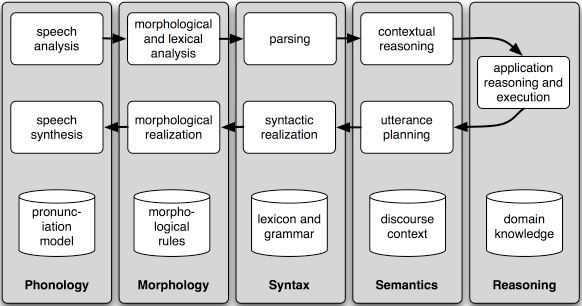
\includegraphics[width=1\textwidth]{pipline}
    \caption{Simple Pipeline Architecture for a Spoken Dialogue System\cite{NLPbook}}
    \label{fig:1}
\end{figure}

In Figure~\ref{fig:1}, \emph{Spoken input (top left) is analyzed, words are recognized, sentences are parsed and interpreted in context, application-specific actions take place (top right); a response is planned, realized as a syntactic structure, then to suitably inflected words, and finally to spoken output; different types of linguistic knowledge inform each stage of the process.}

Dialogue systems give us an opportunity to mention the commonly assumed pipeline for NLP. Figure~\ref{fig:1} shows the architecture of a simple dialogue system. Along the top of the diagram, moving from left to right, is a "pipeline" of some language understanding components. These map from speech input via syntactic parsing to some kind of meaning representation. Along the middle, moving from right to left, is the reverse pipeline of components for converting concepts to speech. These components make up the dynamic aspects of the system. At the bottom of the diagram are some representative bodies of static information: the repositories of language-related data that the processing components draw on to do their work.

\subsection{Textual Entailment}
The challenge of language understanding has been brought into focus in recent years by a public "shared task" called Recognizing Textual Entailment (RTE). The basic scenario is simple. Suppose we want to find evidence to support the hypothesis: \emph{Sandra Goudie was defeated by Max Purnell}, and that we have another short text that seems to be relevant, for example, \emph{Sandra Goudie was first elected to Parliament in the 2002 elections, narrowly winning the seat of Coromandel by defeating Labour candidate Max Purnell and pushing incumbent Green MP Jeanette Fitzsimons into third place}. Does the text provide enough evidence for us to accept the hypothesis? In this particular case, the answer will be "No." We can draw this conclusion easily, but it is very hard to come up with automated methods for making the right decision.
Consequently, some linguistic analysis is crucial. In the previous example, it is important for the system to note that \emph{Sandra Goudie} names the person being defeated in the hypothesis, not the person doing the defeating in the text. As another illustration of the difficulty of the task, consider the following text-hypothesis pair:
\begin{enumerate}[a.]
    \item Text: David Golinkin is the editor or author of eighteen books, and over 150 responsa, articles, sermons and books.
    \item Hypothesis: Golinkin has written eighteen books
    
\end{enumerate}

In order to determine whether the hypothesis is supported by the text, the system needs the following background knowledge: (i) if someone is an author of a book, then he/she has written that book; (ii) if someone is an editor of a book, then he/she has not written (all of) that book; (iii) if someone is editor or author of eighteen books, then one cannot conclude that he/she is author of eighteen books.

\subsection{Information Extraction}
With rise of digital age, there is an explosion of information in the form of news, articles, social media, and so on. Much of this data lies in unstructured form and manually managing and effectively making use of it is tedious, boring and labor intensive. This explosion of information and need for more sophisticated and efficient information handling tools gives rise to Information Extraction(IE) and Information Retrieval(IR) technology. Information Extraction systems takes natural language text as input and produces structured information specified by certain criteria, that is relevant to a particular application. Various sub-tasks of IE such as Named Entity Recognition, Coreference Resolution, Named Entity Linking, Relation Extraction, Knowledge Base reasoning forms the building blocks of various high end Natural Language Processing (NLP) tasks such as Machine Translation, Question-Answering System, Natural Language Understanding, Text Summarization and Digital Assistants like Siri, Cortana and Google Now~\cite{DBLP:journals/corr/abs-1807-02383}.
\begin{figure}[htbp]
    \centering
    \includegraphics[width=.8\textwidth]{ie}
    \caption{Simple Pipeline Architecture for an Information Extraction System~\cite{DBLP:journals/corr/abs-1807-02383}.}
    \label{fig:2}
\end{figure}

Figure~\ref{fig:2} shows the architecture for a simple information extraction system. It begins by processing a document using several of the procedures: first, the raw text of the document is split into sentences using a sentence segmenter, and each sentence is further subdivided into words using a tokenizer. Next, each sentence is tagged with part-of-speech tags, which will prove very helpful in the next step, named entity detection. In this step, we search for mentions of potentially interesting entities in each sentence. Finally, we use relation detection to search for likely relations between different entities in the text.
\subsection{Task Definition}
In our project, we are developing an agent that will follow Bengali instructions to navigate in real-life visual environment.
\begin{itemize}
	\item Inputs: Text based instructions in Bengali language.
	\item Outputs: Mapping instructions and visual observations to actions and execute them in the environment.
\end{itemize}

\section{Motivation}
Computers are great at working with structured data like spreadsheets and database tables. But us humans usually communicate in words, not in tables. That’s unfortunate for computers. A lot of information in the world is unstructured raw text in English or another human language. How can we get a computer to understand unstructured text and extract data from it?

Advances in robotics are enabling progressively more sophisticated, capable technologies to reach large consumer populations. Such systems offer unprecedented potential for AI to help in a variety of human-centric applications such as elder care and household maintenance. However, natural, easy-touse interfaces to such systems, such as those employing natural language, are lagging behind. As robots become more prevalent—and as the need for the services they can offer grows—the importance of allowing non-expert users to interact with them naturally and comfortably increases. Natural language is an excellent modality for end users to give instructions and teach robots about their environments~\cite{ijcai2018-810}. 

As long as computers have been around, programmers have been trying to write programs that understand languages like English. The reason is pretty obvious humans have been writing things down for thousands of years and it would be really helpful if a computer could read and understand all that data. 
NLP is important for scientific, economic, social, and cultural reasons. NLP is experiencing rapid growth as its theories and methods are deployed in a variety of new language technologies. For this reason it is important for a wide range of people to have a working knowledge of NLP. Within industry, this includes people in human-computer interaction, business information analysis, and web software development. Within academia, it includes people in areas from humanities computing and corpus linguistics through to computer science and artificial intelligence~\cite{NLPbook}.

\section{Objectives}
By developing the project, we will learn:
\begin{itemize}
    \item To manipulate large corpora, explore linguistic models and analyze language data.
    \item To use the key concepts from NLP and linguistics to describe and analyse language.
    \item To use data structures and linguistics algorithms in robust language processing software.
    \item To extract knowledge from natural language.
    \item To map instructions from natural language to actions.
    \item To deploy an intelligent agent to execute actions in a particular visual environment.
\end{itemize}






    \chapter{Related Works}
Navigation requires the agent to reason about its relative position to objects and how these relations change as it moves through the environment. While in both learning requires relying on indirect supervision to acquire spatial knowledge and language grounding, for navigation, the training data includes demonstrated actions, and for spatial description resolution, annotated target locations. We have studied the problem of reasoning about natural language instructions to navigate and found some works related to our project.

\section{Talk The Walk~\cite{DBLP:journals/corr/abs-1807-03367}}
They introduce the Talk the Walk, where the aim is for two agents, a “guide” and a “tourist”, to interact with each other via natural language in order to achieve a common goal: having the tourist navigate towards the correct location. The guide has access to a map and knows the target location, but does not know where the tourist is; the tourist has a 360-degree view of the world, but knows neither the target location on the map nor the way to it. The agents need to work together through communication in order to successfully solve the task. An example of the task is given in Figure~\ref{fig:3}. 

\begin{figure}[htbp]
    \centering
    \includegraphics[width=1.1\textwidth]{Tourist}
    \caption{ Example of the Talk The Walk task~\cite{DBLP:journals/corr/abs-1807-03367}}
    \label{fig:3}
\end{figure}
In Figure~\ref{fig:3}:  two agents, a “tourist” and a “guide”, interact with each other via natural language in order to have the tourist navigate towards the correct location. The guide has access to a map and knows the target location but not the tourist location, while the tourist does not have a map and is tasked with navigating a 360-degree street view environment. 
\subsection*{Example:}
Tourist: ACTION:TURNRIGHT ACTION:TURNRIGHT\\ 
Guide: Hello, what are you near?\\ 
Tourist: ACTION:TURNLEFT ACTION:TURNLEFT ACTION:TURNLEFT\\ 
Tourist: Hello, in front of me is a Brooks Brothers \\
Tourist: ACTION:TURNLEFT ACTION:FORWARD ACTION:TURNLEFT ACTION:TURNLEFT 
Guide: Is that a shop or restaurant? \\
Tourist: ACTION:TURNLEFT \\
Tourist: It is a clothing shop.\\ 
Tourist: ACTION:TURNLEFT \\
Guide: You need to go to the intersection in the northwest corner of the map\\ Tourist: ACTION:TURNLEFT\\ 
Tourist: There appears to be a bank behind me.\\ 
Tourist: ACTION:TURNLEFT ACTION:TURNLEFT ACTION:TURNRIGHT ACTION:TURNRIGHT\\ Guide: Ok, turn left then go straight up that road \\
Tourist: ACTION:TURNLEFT ACTION:TURNLEFT ACTION:TURNLEFT ACTION:FORWARD ACTION:TURNRIGHT ACTION:FORWARD ACTION:FORWARD ACTION:TURNLEFT ACTION:TURNLEFT ACTION:TURNLEFT \\
Guide: There should be shops on two of the corners but you need to go to the corner without a shop.\\ 
Tourist: ACTION:FORWARD ACTION:FORWARD ACTION:FORWARD ACTION:TURNLEFT ACTION:TURNLEFT\\ 
Guide: let me know when you get there. \\
Tourist: on my left is Radio city Music hall.\\
Tourist: ACTION:TURNLEFT ACTION:FORWARD ACTION:TURNLEFT ACTION:TURNRIGHT ACTION:TURNRIGHT \\
Tourist: I can’t go straight any further.\\ 
Guide: ok. turn so that the theater is on your right.\\ 
Guide: then go straight \\
Tourist: That would be going back the way I came \\
Guide: yeah. I was looking at the wrong bank \\
Tourist: I’ll notify when I am back at the brooks brothers, and the bank.\\ Tourist: ACTION:TURNRIGHT \\
Guide: make a right when the bank is on your left \\
Tourist: ACTION:FORWARD ACTION:FORWARD ACTION:TURNRIGHT \\
Tourist: Making the right at the bank. \\
Tourist: ACTION:FORWARD ACTION:FORWARD \\
Tourist: I can’t go that way. \\
Tourist: ACTION:TURNLEFT \\
Tourist: Bank is ahead of me on the right \\
Tourist: ACTION:FORWARD ACTION:FORWARD ACTION:TURNLEFT \\
Guide: turn around on that intersection \\
Tourist: I can only go to the left or back the way I just came. \\
Tourist: ACTION:TURNLEFT \\
Guide: you’re in the right place. do you see shops on the corners? \\
Guide: If you’re on the corner with the bank, cross the street \\
Tourist: I’m back where I started by the shop and the bank. \\
Tourist: ACTION:TURNRIGHT \\
Guide: on the same side of the street? \\
Tourist: crossing the street now \\
Tourist: ACTION:FORWARD ACTION:FORWARD ACTION:TURNLEFT \\
Tourist: there is an I love new york shop across the street on the left from me now \\
Tourist: ACTION:TURNRIGHT ACTION:FORWARD \\
Guide: ok. I’ll see if it’s right. \\
Guide: EVALUATE LOCATION \\
Guide: It’s not right. \\
Tourist: What should I be on the look for? \\
Tourist: ACTION:TURNRIGHT ACTION:TURNRIGHT ACTION:TURNRIGHT \\
Guide: There should be shops on two corners but you need to be on one of the corners without the shop. \\
Guide: Try the other corner. \\
Tourist: this intersection has 2 shop corners and a bank corner \\
Guide: yes. that’s what I see on the map. \\
Tourist: should I go to the bank corner? or one of the shop corners? or the blank corner (perhaps a hotel) \\
Tourist: ACTION:TURNLEFT ACTION:TURNLEFT ACTION:TURNRIGHT ACTION:TURNRIGHT Guide: Go to the one near the hotel. The map says the hotel is a little further down but it might be a little off. \\
Tourist: It’s a big hotel it’s possible. \\
Tourist: ACTION:FORWARD ACTION:TURNLEFT ACTION:FORWARD ACTION:TURNRIGHT\\ Tourist: I’m on the hotel corner \\
Guide: EVALUATE LOCATION\\

Talk The Walk is the first task to bring all three aspects together: perception for the tourist observing the world, action for the tourist to navigate through the environment, and interactive dialogue for the tourist and guide to work towards their common goal.

As the main focus of their task is on interactive dialogue, they limit the difficulty of the control problem by having the tourist navigating a 2D grid via discrete actions (turning left, turning right and moving forward)~\cite{DBLP:journals/corr/abs-1807-03367}.
 
 
    \section{Mapping Instructions and Visual Observations to Actions~\cite{DBLP:journals/corr/MisraLA17}}
They propose to directly map raw visual observations and text input to actions for instruction execution.  While existing approaches assume access to structured environment representations or use a pipeline of separately trained models, they learn a single model to jointly reason about linguistic and visual input. They use reinforcement learning in a contextual bandit setting to train a neural network agent. To guide the agent’s exploration, they use reward shaping with different forms of supervision~\cite{DBLP:journals/corr/MisraLA17}.

\begin{figure}[htbp]
    \centering
    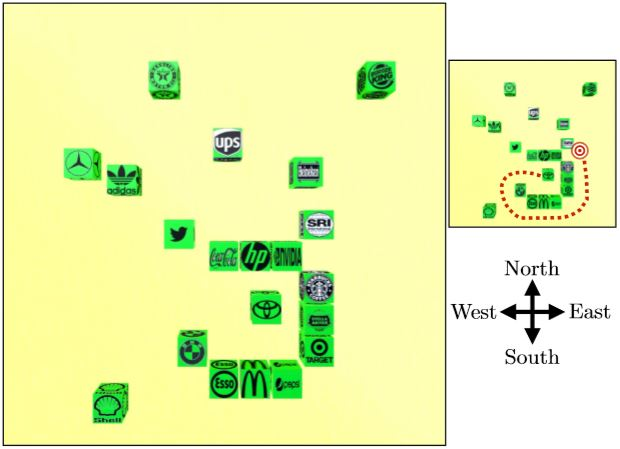
\includegraphics[width=.8\textwidth]{block}
    \caption{Blocks environment}
\end{figure}
\newpage
\begin{table}[h!]
    \begin{tabular}{|p{15cm}|}
    \hline
    Put the Toyota block in the same row as the SRI block, in the first open space to the right of the SRI block.\\
    \hline
    Move Toyota to the immediate right of SRI, evenly aligned and slightly separated.\\
    \hline
    Move the Toyota block around the pile and place it just to the right of the SRI block.\\
    \hline
    Place Toyota block just to the right of The SRI Block.\\
    \hline
    Toyota, right side of SRI.\\
    \hline
    \end{tabular}
    \caption{Instructions in the Blocks environment}
    \label{tab:1}
\end{table}

In Table~\ref{tab:1}, illustrates the problem in the Blocks environment. The agent observes the environment as an RGB image using a camera sensor. Given the RGB input, the agent must recognize the blocks and their layout. To understand the instruction, the agent must identify the block to move (Toyota block) and the destination (just right of the SRI block). This requires solving semantic and grounding problems. For example, consider the topmost instruction in the figure. The agent needs to identify the phrase referring to the block to move, Toyota block, and ground it. It must resolve and ground the phrase SRI block as a reference position, which is then modified by the spatial meaning recovered from the same row as or first open space to the right of, to identify the goal position. Finally, the agent needs to generate actions, for example moving the Toyota block around obstructing blocks. 

To address these challenges with a single model, they design a neural network agent. The agent executes instructions by generating a sequence of actions. At each step, the agent takes as input the instruction text, observes the world as an RGB image, and selects the next action. Action execution changes the state of the world. Given an observation of the new world state, the agent selects the next action. This process continues until the agent indicates execution completion. When selecting actions, the agent jointly reasons about its observations and the instruction text. This enables decisions based on close interaction between observations and linguistic input.

They study the problem of learning to execute instructions in a situated environment given only raw visual observations. Supervised approaches do not explore adequately to handle test time errors, and reinforcement learning approaches require a large number of samples for good convergence. Their solution provides an effective combination of both approaches: reward shaping to create relatively stable optimization in a contextual bandit setting.

This combination is designed for a few-samples regime, as we address. When the number of samples is unbounded, the drawbacks observed in this scenario for optimizing longer term reward do not hold.

    \section{Vision-and-Language Navigation}
The idea in~\cite{DBLP:journals/corr/abs-1711-07280} that they might be able to provide general, verbal directions to a robot and have a minimum of an affordable likelihood that it'll do the specified task is one in all the long-held goals of artificial intelligence, and robots.
Despite vital progress, there area unit variety of major technical challenges that require to be over precede robots are going to be able to perform general tasks within the universe. One in all the first needs are going to be new techniques for linking language to vision and action in \emph{unstructured}, \emph{previously unseen environments}. They refer it as Vision-and-Language Navigation (VLN) because of the navigation version of this challenge~\cite{DBLP:journals/corr/abs-1711-07280}.

\begin{figure}[htbp]
    \centering
    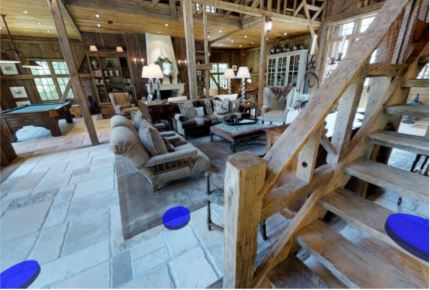
\includegraphics[width=.8\textwidth]{vln}
    \caption{Room-to-Room (R2R) navigation task~\cite{DBLP:journals/corr/abs-1711-07280}}
\end{figure}
\newpage
\subsection*{Instruction}
Head upstairs and walk past the piano through an entryway directly before. Turn right once corridor ends at footage and table. Wait by the moose antlers hanging on the wall.\\

Previous approaches to natural language command of robots have often neglected the visual information processing aspect of the problem. The R2R dataset is the first dataset to evaluate the capability to follow natural language navigation instructions in previously unseen real images at building scale. To explore this task they investigated several baselines and a sequence-to-sequence neural network agent.  The process used to generate R2R is applicable to a host of related vision and language problems, particularly in robotics. 

    \section{Enabling Robots to Understand Incomplete Natural Language Instructions Using Commonsense Reasoning}
In~\cite{DBLP:journals/corr/TesslerGZMM16}, they introduce Language-Model-based commonsense Reasoning (LMCR), a replacement technique that permits a robot to concentrate to a linguistic communication instruction from a person's, observe the surroundings around it, and mechanically fill in info missing from the instruction mistreatment environmental context and a replacement common sensible reasoning approach. Their approach initial converts associate degree instruction provided as free linguistic communication into a type that a robot will perceive by parsing it into verb frames.

\begin{figure}[htbp]
    
    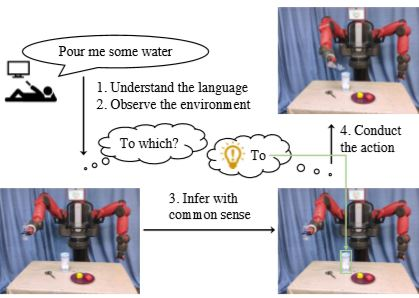
\includegraphics[width=.8\textwidth]{enable}
    \caption{A natural language controlled robot employing commonsense knowledge to interpret an instruction with missing information~\cite{DBLP:journals/corr/TesslerGZMM16} }
    \label{fig:enable}
\end{figure}
\newpage
Their approach then fills in missing data inside the instruction by observant objects in its neck of the woods and finance common wise reasoning. To be told common wise reasoning automatically, their approach distills data from huge unstructured matter corpora by coaching job a language model. Our results show the reasonableness of a automaton learning common wise data automatically from web-based matter corpora, and additionally the facility of learned common wise reasoning models in serving to a automaton to autonomously perform tasks supported incomplete communication directions.

A person provide instruction “pour him some water” however the automaton cannot perform the action while not knowing wherever to pour. When scanning the surroundings, the robot uses common sensible information to work out the missing parameters and with success perform the action.


    
    \section{Methodology}	
When dealing with natural language, our main purpose is to make computer understand the rules and formation of
natural language. How a sentence built and how each parts of the sentences are connected with each other. To make computer understand about the human level natural language, we have to design a Natural Language Processing(NLP) Pipeline.\\ 
	
After understanding the given text, we have to make choices that how could we do the task that is instructed in the text. So we need a learning environment by which we can teach our agent(robot) to execute the task. Our task
here is to generate the necessary actions to accomplish the task.\\
	
As in this work we're navigating a robot via natural language instruction, so we also need an environment
where we can view and observe the environment around the robot and give instructions in accordance.\\
	
So in this work our methodology is centered on three key point: A NLP Pipeline, A Learning Algorithm and A Navigation Environment. \\

\subsection{Work Already Done}

\subsubsection{NLP Pipeline Designing}

The first stage of our work is the designing of a NLP pipeline. The steps associated with designing a NLP pipeline are as follows: \\

\begin{enumerate}
    \item Sentence Segmentation
    \item Word Tokenization
    \item Predicting Parts of Speech for Each Token
    \item Text Lemmatization
    \item Identifying Stop Words
    \item Dependency Parsing
    \begin{enumerate}
        \item Finding Noun Phases
    \end{enumerate}
    \item Named Entity Recognition (NER)
\end{enumerate}
\vline

Now we should focus on a brief discussion of these steps. We consider the sentence: "Go near the red triangle. Wait for three seconds. Then go to green rectangle."\\

\paragraph{Sentence Segmentation}
The first step in the pipeline is to break the text apart into separate sentences. Thus gives us this:
\begin{enumerate}
    \item "Go near the red triangle."
    \item "Wait for three seconds."
    \item "Then go to green rectangle."
\end{enumerate}

\paragraph{Word Tokenization}
Now that we’ve split our document into sentences, we can process them one at a time. The next step in our pipeline is to break this sentence into separate words or tokens. This is called tokenization. This is the result: \\

\begin{tabular}{|p{10cm}}
    "Go", "near", "the", "red", "triangle", "." 
\end{tabular}\\
\vline


Tokenization is easy to do in English. We’ll just split apart words whenever there’s a space between them. And we’ll also treat punctuation marks as separate tokens since punctuation also has meaning.

\paragraph{Predicting Parts of Speech for Each Token}
Next, we'll look at each token and try to guess its part of speech-whether it is a noun, a verb, an adjective and so on. Knowing the role of each word in the sentence will help us start to figure out what the sentence is talking about.\\

We can do this by feeding each word (and some extra words around it for context) into a pre-trained part-of-speech classification model. The part-of-speech model was originally trained by feeding it millions of English sentences with each word’s part of speech already tagged and having it learn to replicate that behavior.\\

After processing the whole sentence, we'll have result like this:
\begin{table}[h]
    \centering
    \begin{tabular}{ccccc}
        Go   & near      & the        & red  & triangle \\
        Verb & Adjective & Determiner & Noun & Noun    
    \end{tabular}
\end{table}

\paragraph{Text Lemmatization}
In English (and most languages), words appear in different forms. When working with text in a computer, it is helpful to know the base form of each word so that we know both sentences are talking about the same concept. In NLP, we call finding this process lemmatization-figuring out the most basic form or lemma of each word in the sentence. The same thing applies to verbs. We can also lemmatize verbs by finding their root, unconjugated form. Lemmatization is typically done by having a look-up table of the lemma forms of words based on their part of speech and possibly having some custom rules to handle words that we’ve never seen before.
\paragraph{Identifying Stop Words}
Next, we want to consider the importance of a each word in the sentence. English has a lot of filler words that appear very frequently like “and”, “the”, and “a”. When doing statistics on text, these words introduce a lot of noise since they appear way more frequently than other words. Some NLP pipelines will flag them as stop words —that is, words that you might want to filter out before doing any statistical analysis.

\paragraph{Dependency Parsing}
The next step is to figure out how all the words in our sentence relate to each other. This is called dependency parsing.\\

The goal is to build a tree that assigns a single parent word to each word in the sentence. The root of the tree will be the main verb in the sentence.\\

It’s also important to remember that many English sentences are ambiguous and just really hard to parse. In those cases, the model will make a guess based on what parsed version of the sentence seems most likely but it’s not perfect and sometimes the model will be embarrassingly wrong. But over time our NLP models will continue to get better at parsing text in a sensible way.
\subparagraph{Finding Noun Phrases}
So far, we’ve treated every word in our sentence as a separate entity. But sometimes it makes more sense to group together the words that represent a single idea or thing. We can use the information from the dependency parse tree to automatically group together words that are all talking about the same thing.

\paragraph{Named Entity Recognition (NER)}
The goal of Named Entity Recognition, or NER, is to detect and label the nouns with the real-world concepts that they represent. But NER systems aren’t just doing a simple dictionary lookup. Instead, they are using the context of how a word appears in the sentence and a statistical model to guess which type of noun a word represents.\\

Here are just some of the kinds of objects that a typical NER system can tag: People’s names, Company names, Geographic locations (Both physical and political), Product names, Dates and times, Amounts of money, Names of events.\\
In our environment we'll tag certain locations of the environment.\\


\subsubsection{Action Generation}
For navigating in the environment, our agent has to develop or generate actions for the given instructions. Currently we use the basic reinforcement learning algorithm: Value Iteration to generate actions for the agent.\\

Value Iteration algorithm works in a grid environment where we've one or more rewards and one or more punishments in some grids. According to that reward or punishment we generate value for each action for each grid. The formula associated with value iteration algorithm is as follows:\\

$V^*(s) = \max \sum T(s, a, s')[R(s, a, s')  + \gamma V^*(s')]$\\

An example of a $3 X 3$ grid with optimal policy and optimal values after applying value iteration is given in the following image.\\


\begin{figure}[ht]
    \centering
    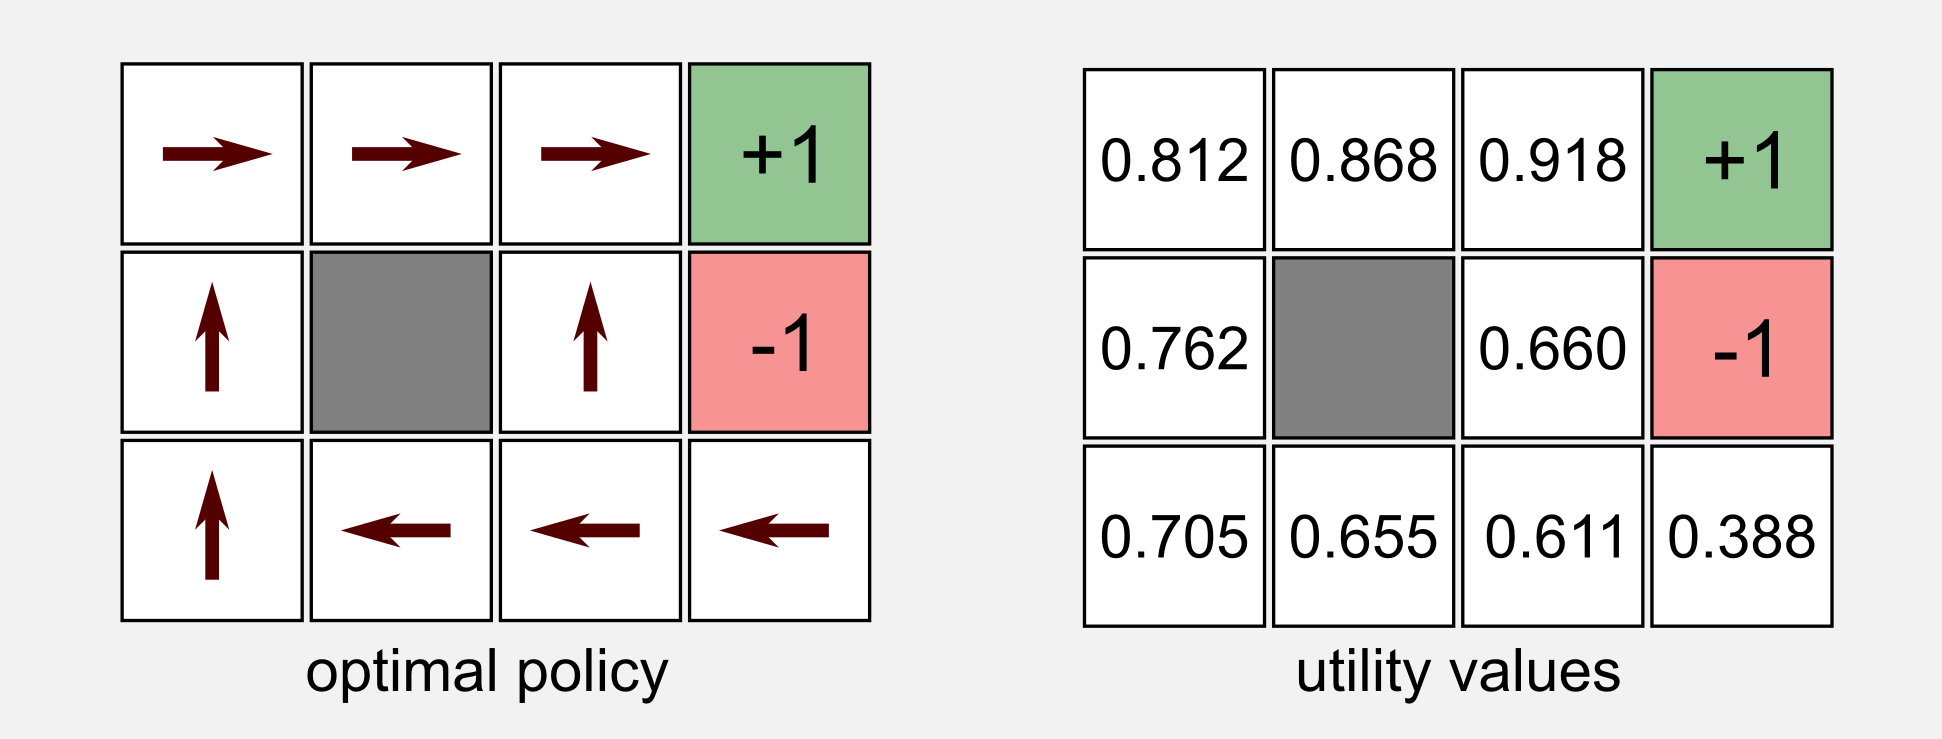
\includegraphics[scale=0.5]{value_iteration}
    \caption{Value Iteration Example}
\end{figure}
\vline

For using the Value Iteration algorithm we split our environment in $25 X 35$ grids. We set reward in grids which is our destinations. We decrease reward value according to the hierarchy or the destination. Similarly we set negative reward in the grid that we should have to avoid.\\

After iterating the algorithm over the whole grid several time we can get the optimal action for each grid. According to this optimal option, agent(robot) will start moving.\\


\subsubsection{Environment Designing}
For now we've used a simple graphical interface to describe the environment and observe the movement of the agent. We should give navigation instruction according to the given environment.

\begin{figure}[h]
    \centering
    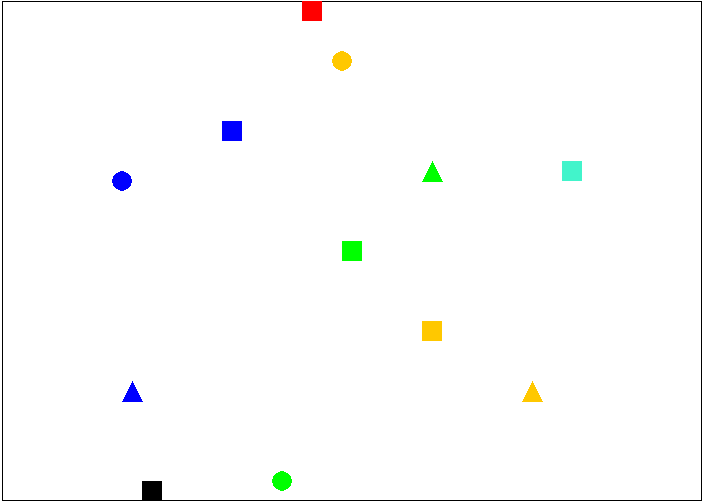
\includegraphics[scale=0.5]{environment}
    \caption{Currently Used Environment}
\end{figure}
\vline

\subsection{Expected Work to be Done}

\subsubsection{NLP Pipeline Designing}
What pipeline we've already designed is moderately enough for language processing tasks. We didn't use the whole pipeline as our used navigation environment is still not much complex. With the increasing complexity of the navigation environment, input instructions will be complex. So for our upgraded version of this project we'll need this whole NLP pipeline.\\

We've designed our NLP pipeline for English language. But as our project aims to navigate robot using Bengali language, we've needed some special consideration for Bengali NLP pipeline. We've to convert the whole pipeline such a way that it could process Bengali language.


\subsubsection{Action Generation}
We aim to develop a Machine Learning model to generate action from a given instruction. This is the core part of our project. For training machine learning model we need data of our environment. As we still didn't design the complex and complete environment we don't have those data right now.\\

After completing the designing of the environment, we use the navigation instruction data to to train our model to generate actions.

\subsubsection{Environment Designing}
We want to design an environment with real life element like tree, building etc. We want to represent the environment via a graphical interface.\\

Alongside the graphical interface we also demonstrate the environment in real life with some dummy element like toy car or toy tree. We want to synchronize the navigation of real life demo in our graphical interface too.\\

After completing the design of the environment and above mentioned two other steps we hope to have our project ready completely. 
	
    \chapter{Comparative Result}
	
	\section{Used Model's Performance}
	As described in $Methodology$ section, we've used LSTM model here. A quick summery of LSTM performance is as follow. \\
	
	\begin{table}[H]
		\centering
		\begin{tabular}{|l|l|}
			\hline
			Accuracy Type       & Accuracy \\ \hline
			Train Accuracy      & 89.72\%  \\ \hline
			Validation Accuracy & 97.78\%  \\ \hline
			Test Accuracy       & 97.90\%  \\ \hline
		\end{tabular}
		\caption{LSTM Accuracy}
	\end{table}
	
	
	The following figure shows the graph of model's loss during 5 epochs.\\
	
	\begin{figure}[H]
		\centering
		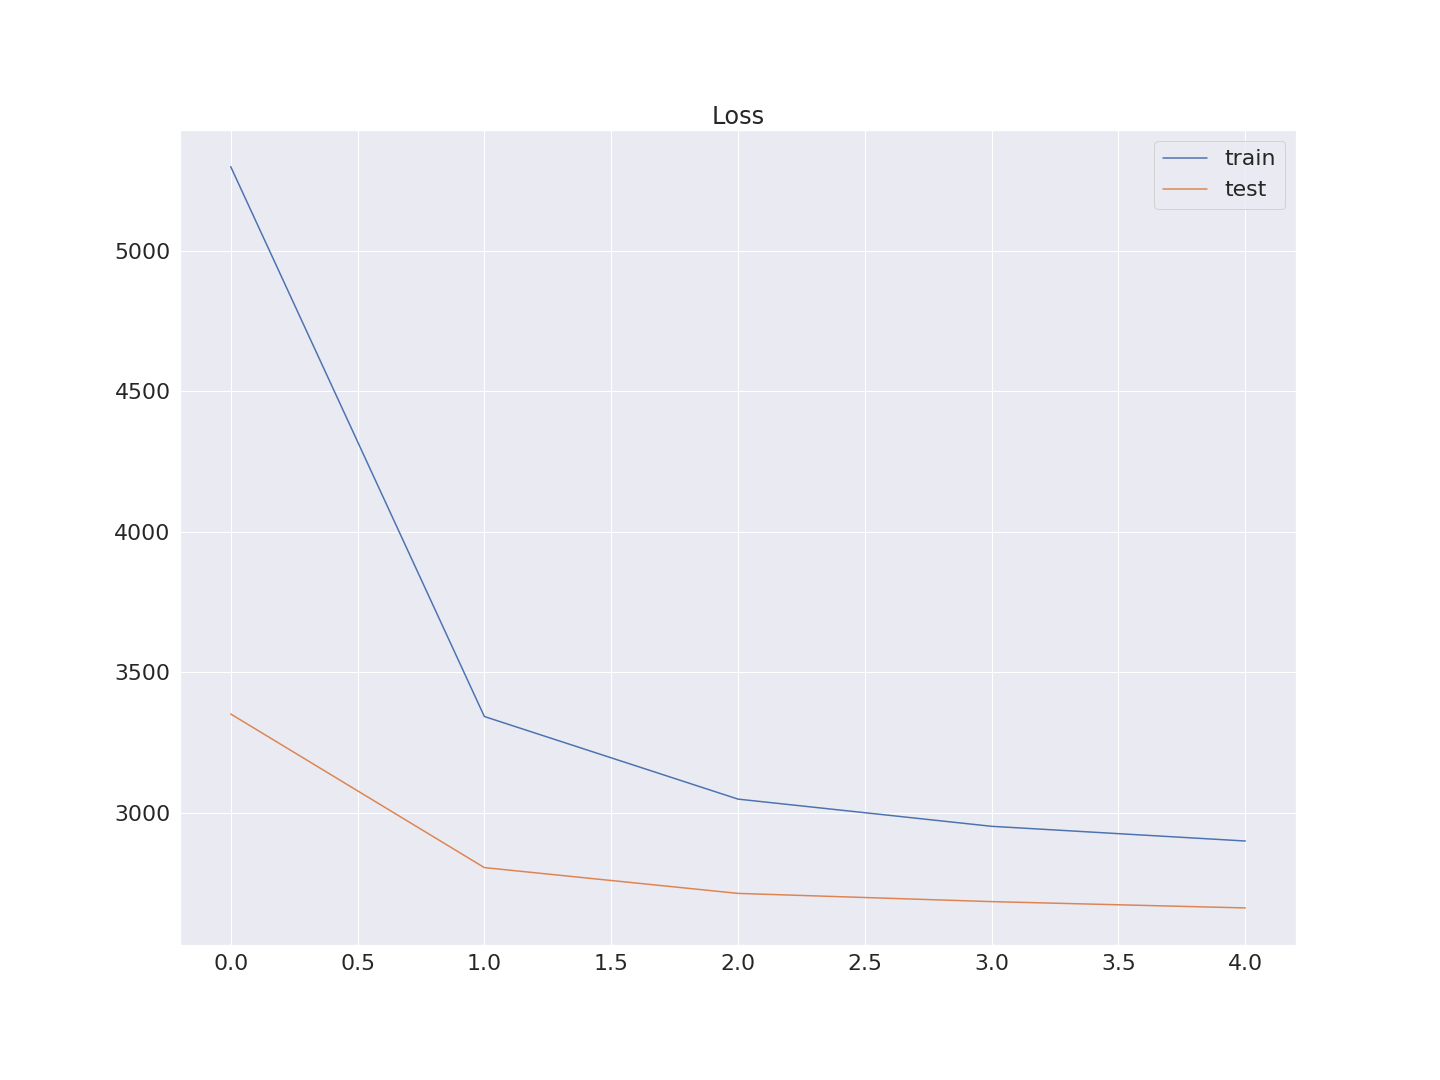
\includegraphics[scale=0.30]{lstm_loss}
		\caption{LSTM Loss Graph}
	\end{figure}
	\vline

	The following figure shows the graph of the model's test accuracy during 5 epochs.\\
	\begin{figure}[H]
		\centering
		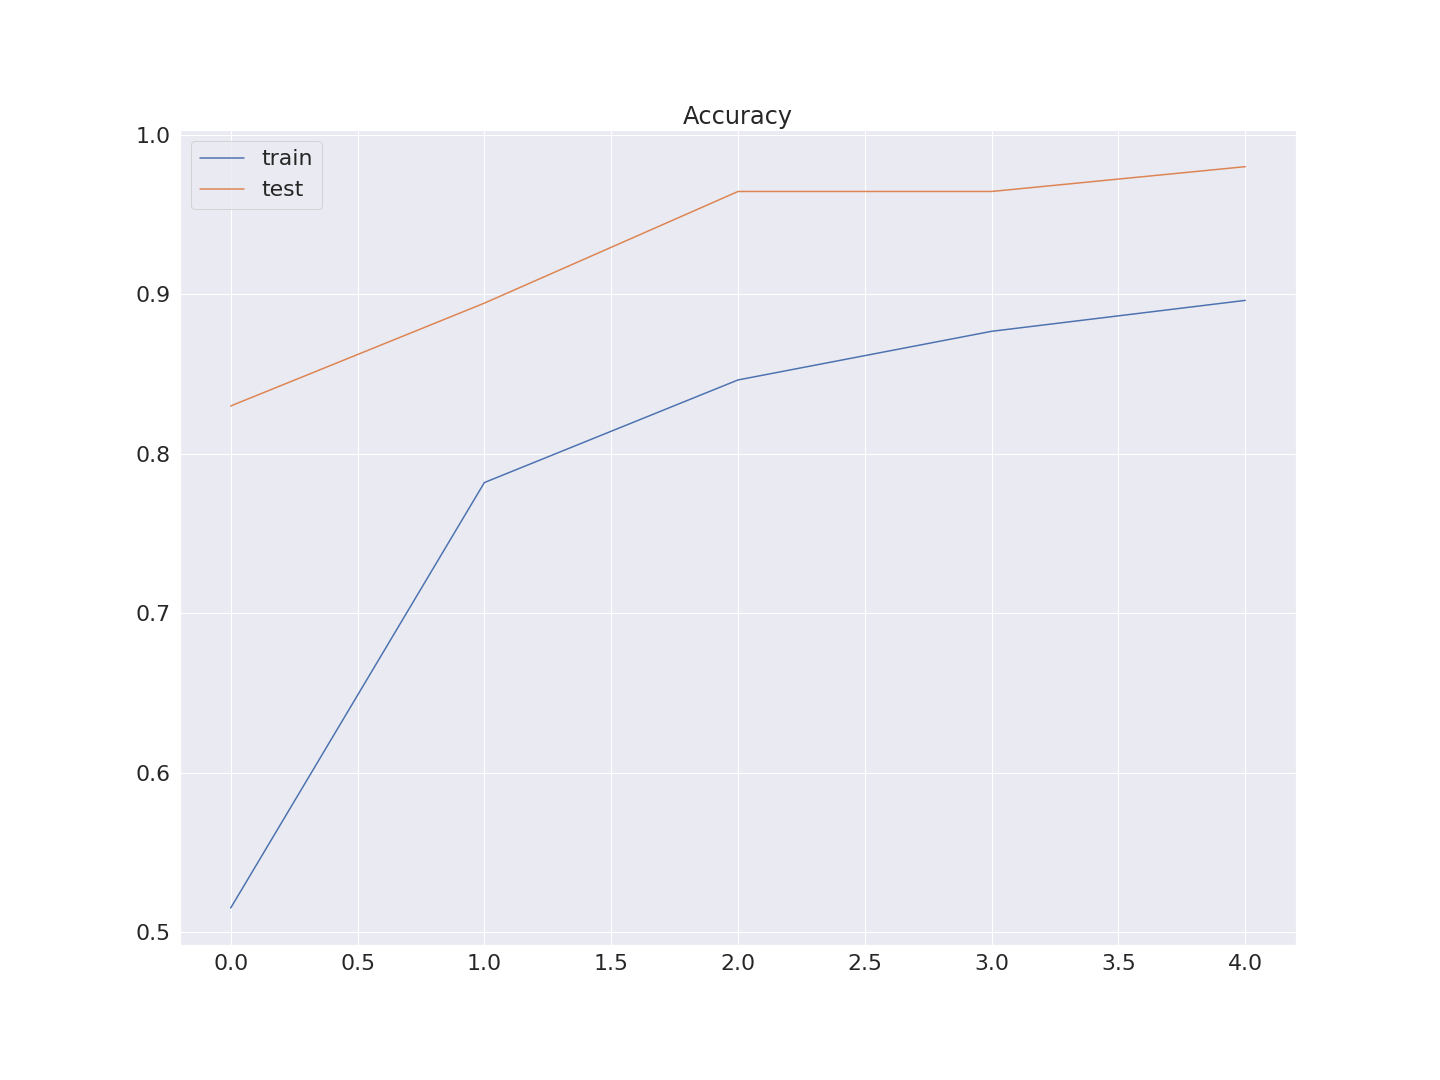
\includegraphics[scale=0.30]{lstm_accuracy}
		\caption{LSTM Accuracy Graph}
	\end{figure}
	\vline
	
	
	\section{Another Model's Performance}
	We try with other two model architecture, RNN and GRU. Here we'll look the performance of these two model. \\
	
		\subsection{RNN Performance}
		A quick summery of RNN model performance is as follow. \\
		
		\begin{table}[H]
			\centering
			\begin{tabular}{|l|l|}
				\hline
				Accuracy Type       & Accuracy \\ \hline
				Train Accuracy      & 57.53\%  \\ \hline
				Validation Accuracy & 63.00\%  \\ \hline
				Test Accuracy       & 63.00\%  \\ \hline
			\end{tabular}
			\caption{RNN Accuracy}
		\end{table}
		
		
		The following figure shows the graph of RNN's loss during 5 epochs.\\
		
		\begin{figure}[H]
			\centering
			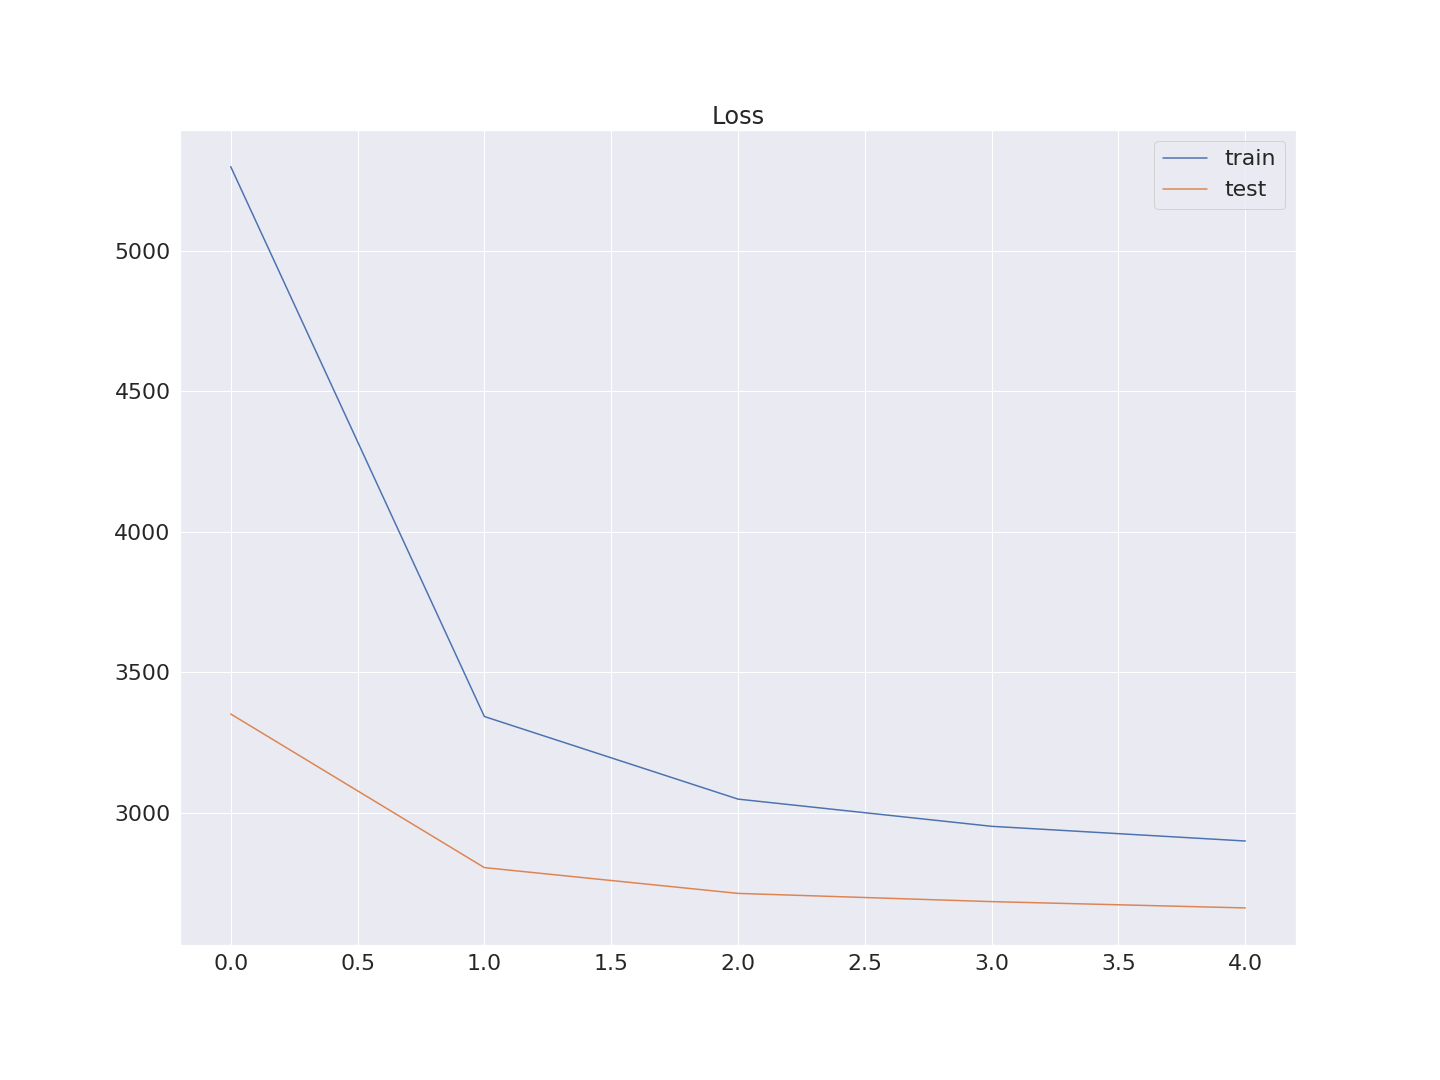
\includegraphics[scale=0.30]{rnn_loss}
			\caption{RNN Loss Graph}
		\end{figure}
		\vline
		
		The following figure shows the graph of RNN's test accuracy during 5 epochs.\\
		\begin{figure}[H]
			\centering
			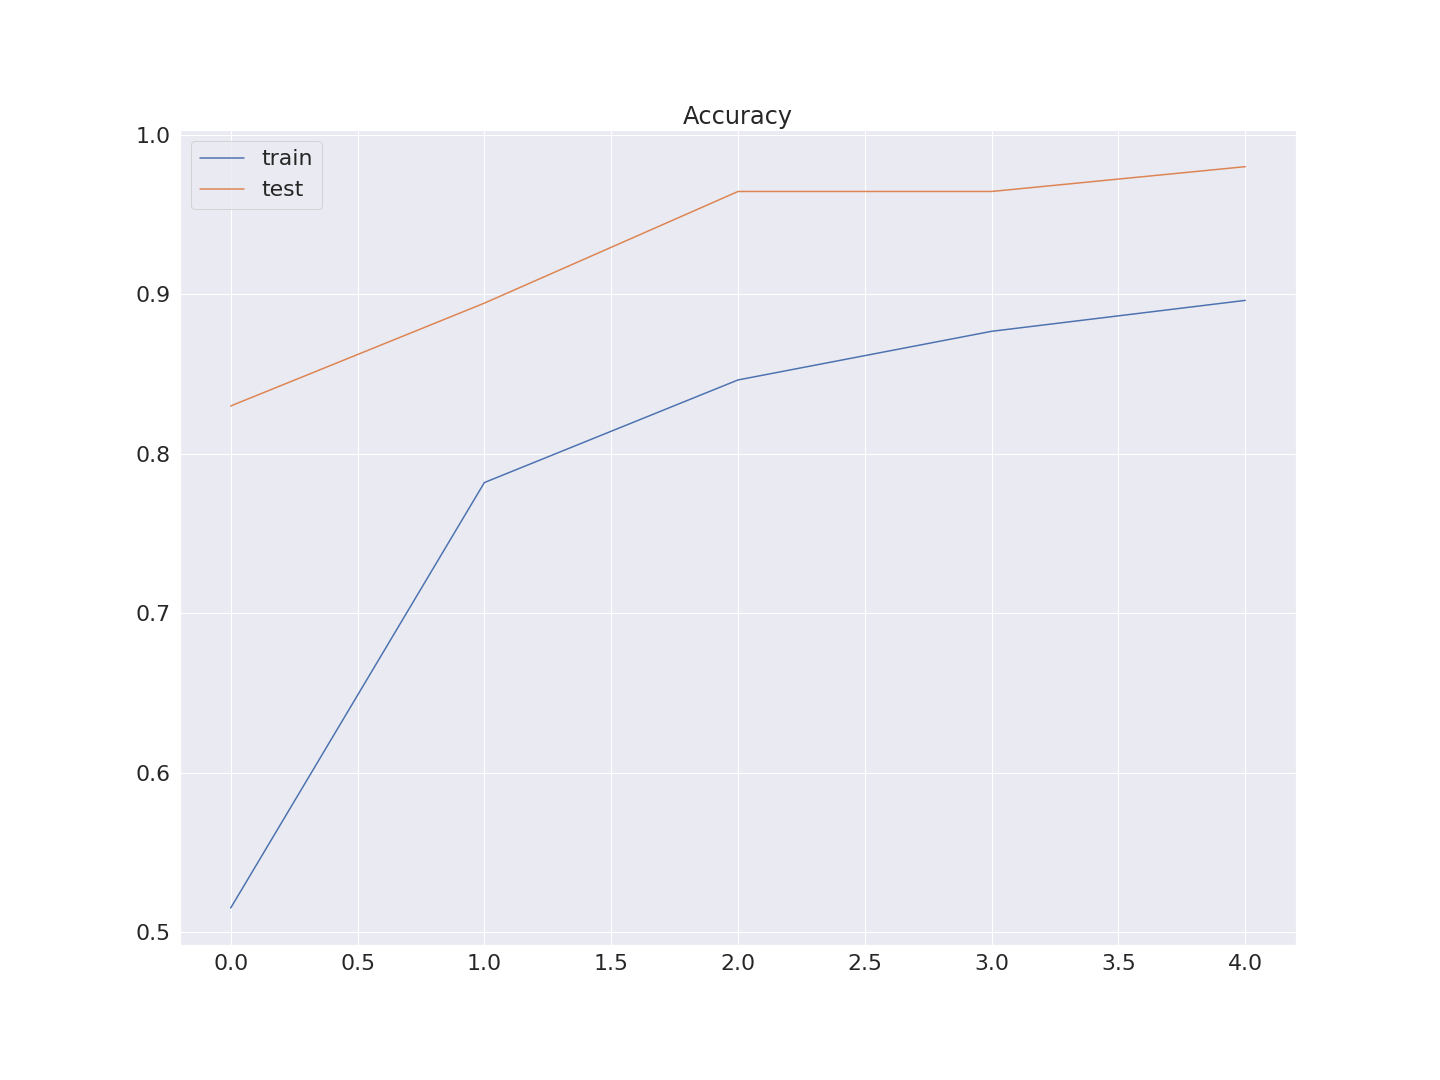
\includegraphics[scale=0.30]{rnn_accuracy}
			\caption{RNN Accuracy Graph}
		\end{figure}
		\vline
		
		
		\subsection{GRU Performance}
		A quick summery of GRU model performance is as follow. \\
		
		\begin{table}[H]
			\centering
			\begin{tabular}{|l|l|}
				\hline
				Accuracy Type       & Accuracy \\ \hline
				Train Accuracy      & 83.59\%  \\ \hline
				Validation Accuracy & 37.30\%  \\ \hline
				Test Accuracy       & 37.30\% \\ \hline
			\end{tabular}
			\caption{GRU Accuracy}
		\end{table}
		
		
		The following figure shows the graph of GRU's loss during 5 epochs.\\
		
		\begin{figure}[H]
			\centering
			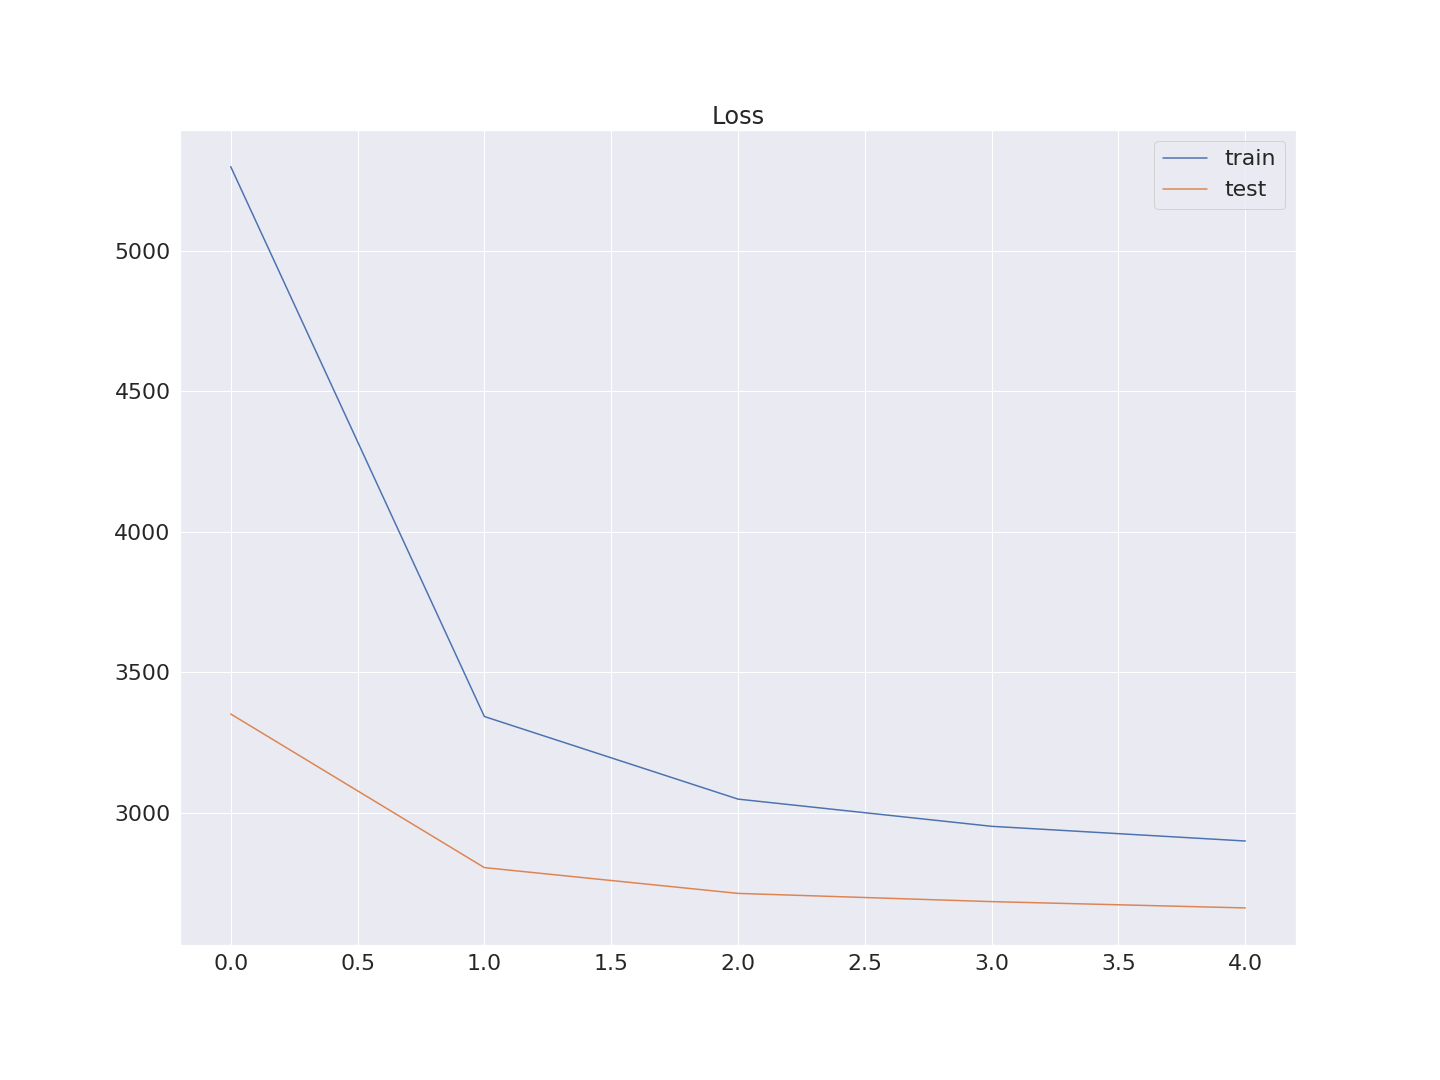
\includegraphics[scale=0.30]{gru_loss}
			\caption{GRU Loss Graph}
		\end{figure}
		\vline
		
		The following figure shows the graph of GRU's test accuracy during 5 epochs.\\
		\begin{figure}[H]
			\centering
			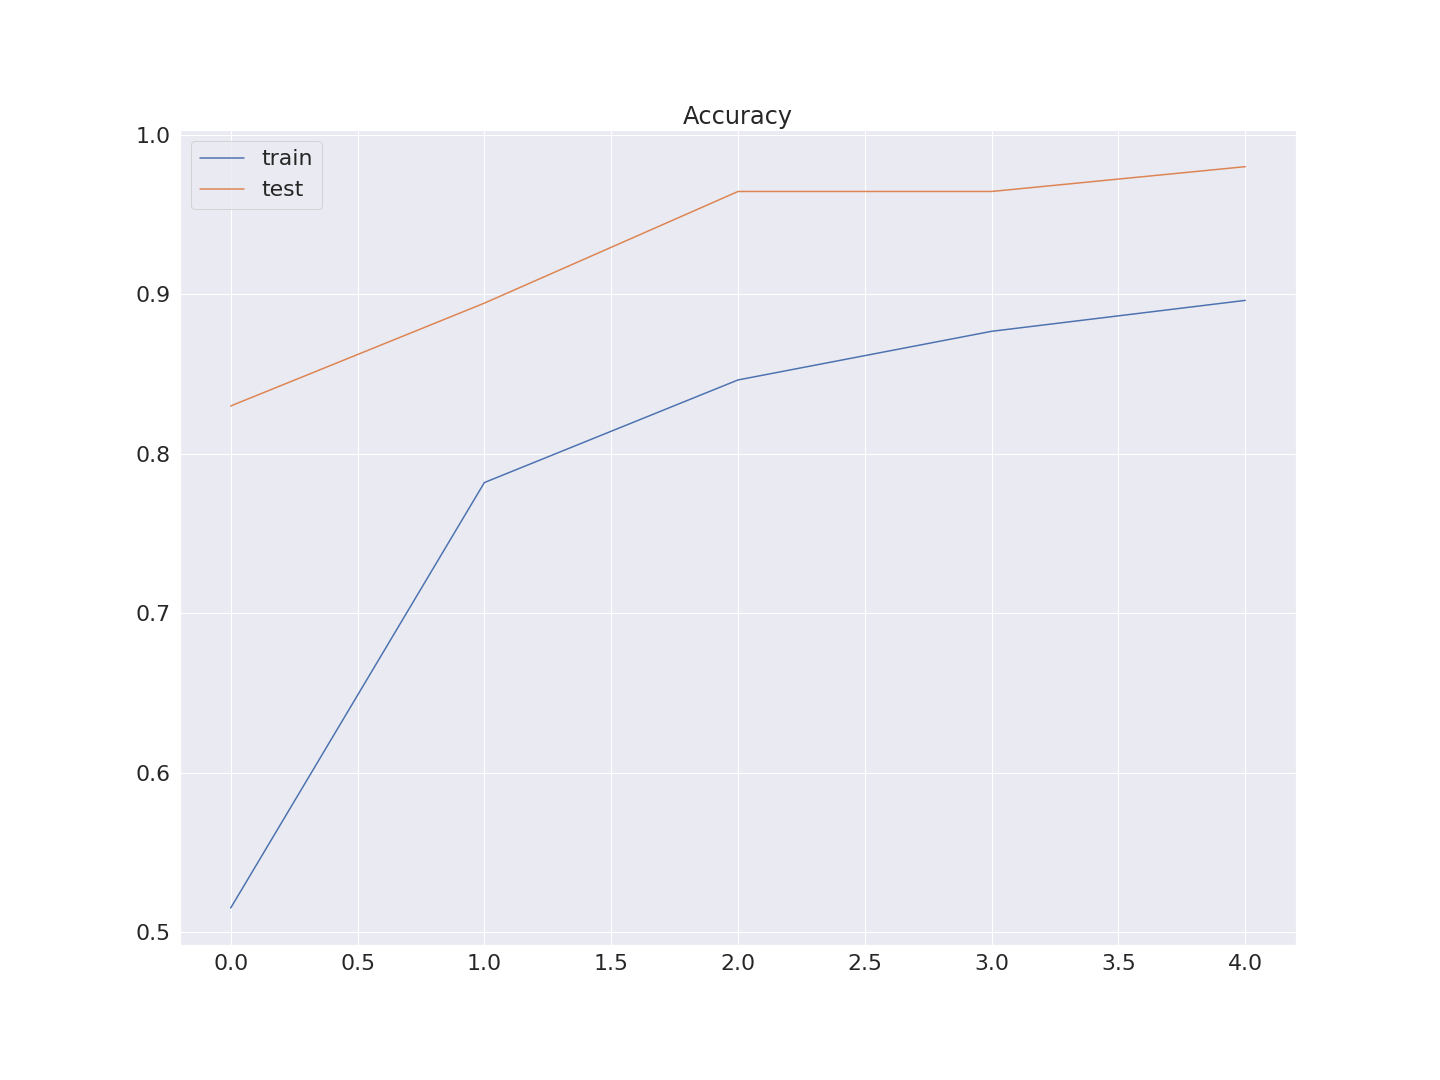
\includegraphics[scale=0.30]{gru_accuracy}
			\caption{GRU Accuracy Graph}
		\end{figure}
		\vline
		
	
	\section{Comparison Altogether}
	Lets have look on both of these model and their accuracy altogether. \\
	
	\begin{table}[H]
		\centering
		\begin{tabular}{|l|l|l|l|}
			\hline
			Accuracy Type \textbackslash Model & LSTM    & RNN     & GRU     \\ \hline
			Train Accuracy                     & 89.72\% & 57.53\% & 83.59\% \\ \hline
			Validation Accuracy                & 97.78\% & 63.00\% & 37.30\% \\ \hline
			Test Accuracy                      & 97.90\% & 63.00\% & 37.30\% \\ \hline
		\end{tabular}
		\caption{Accuracy Comparison Between LSTM, RNN and GRU}
	\end{table}
	
	The table above shows various accuracy comparison between various models. And we can easily see that LSTM is the obvious champion here.
    \chapter{Simulation}
	We provided the initial output in a web interface. The following figure shows the first appearance of our simulation environment when we access to the local server. \\
	
	\begin{figure}[H]
		\centering
		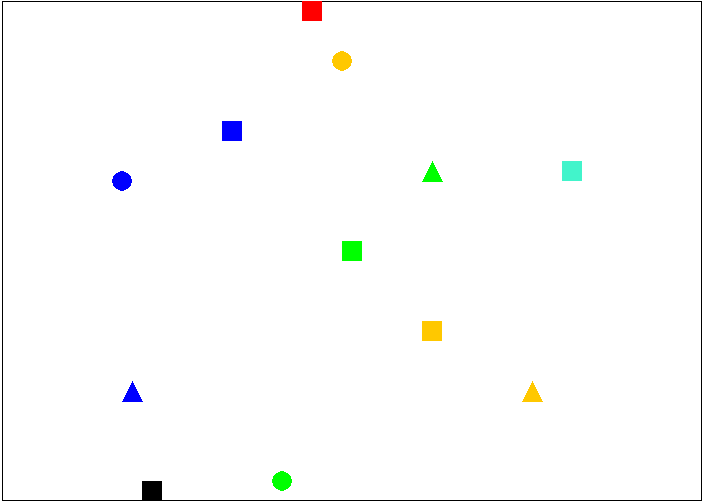
\includegraphics[scale=0.30]{environment}
		\caption{First Appearance of the Environment}
	\end{figure}
	\vline
	
	The instruction we give in voice not all are properly detected by our used speech recognition module. In this simulation we modified the detected text here.\\
	
	If we give voice instruction: `Go from Cruzon Hall to TSC through Shaheed Minar', the output in the environment will look like as follow. \\
	\begin{figure}[H]
		\centering
		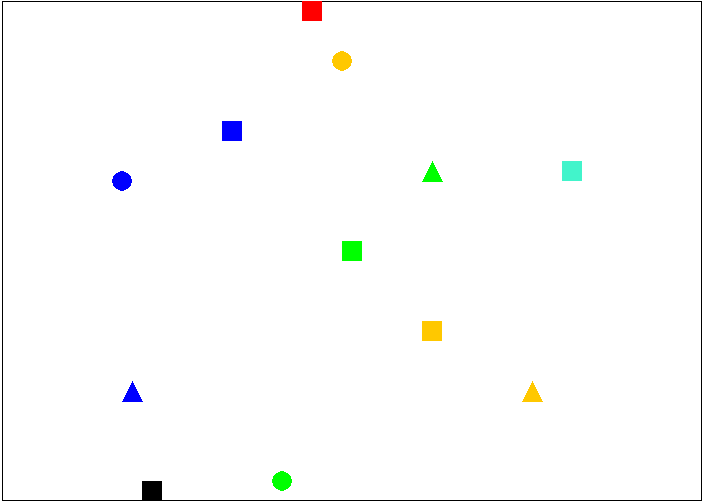
\includegraphics[scale=0.30]{environment}
		\caption{Output for an Instruction}
	\end{figure}
	\vline
	
	As the models sometimes makes error, here is a erroneous case. For instruction `Go from Bangla Academy to Dhaka Medical college through Shahidullah Hall', the model detected Dhaka Medical College as source instead of destination and similarly detect Bangla Academy as destination instead of source. \\
	\begin{figure}[H]
		\centering
		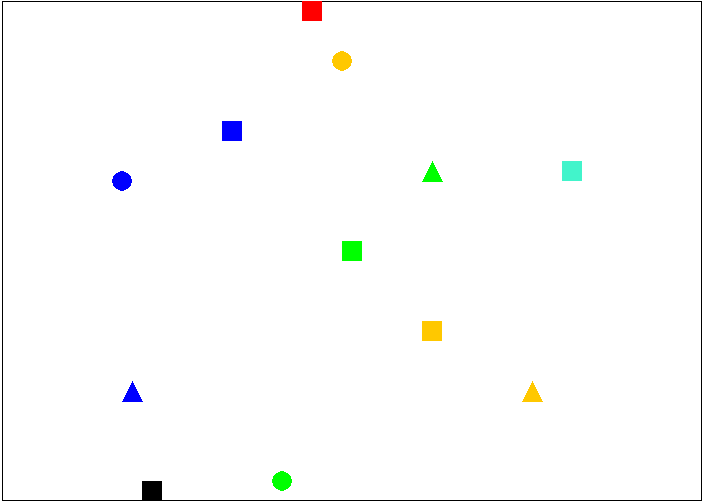
\includegraphics[scale=0.30]{environment}
		\caption{Output for an Instruction}
	\end{figure}
	\vline
	
	\textbf{Hardware} \\
	We also have designed a simple line following robot which is able to follow the instruction we gave in voice. We make a dummy track where the robot assumes some node as some real location. The following figure shows our designed line following robot.
	\begin{figure}[H]
		\centering
		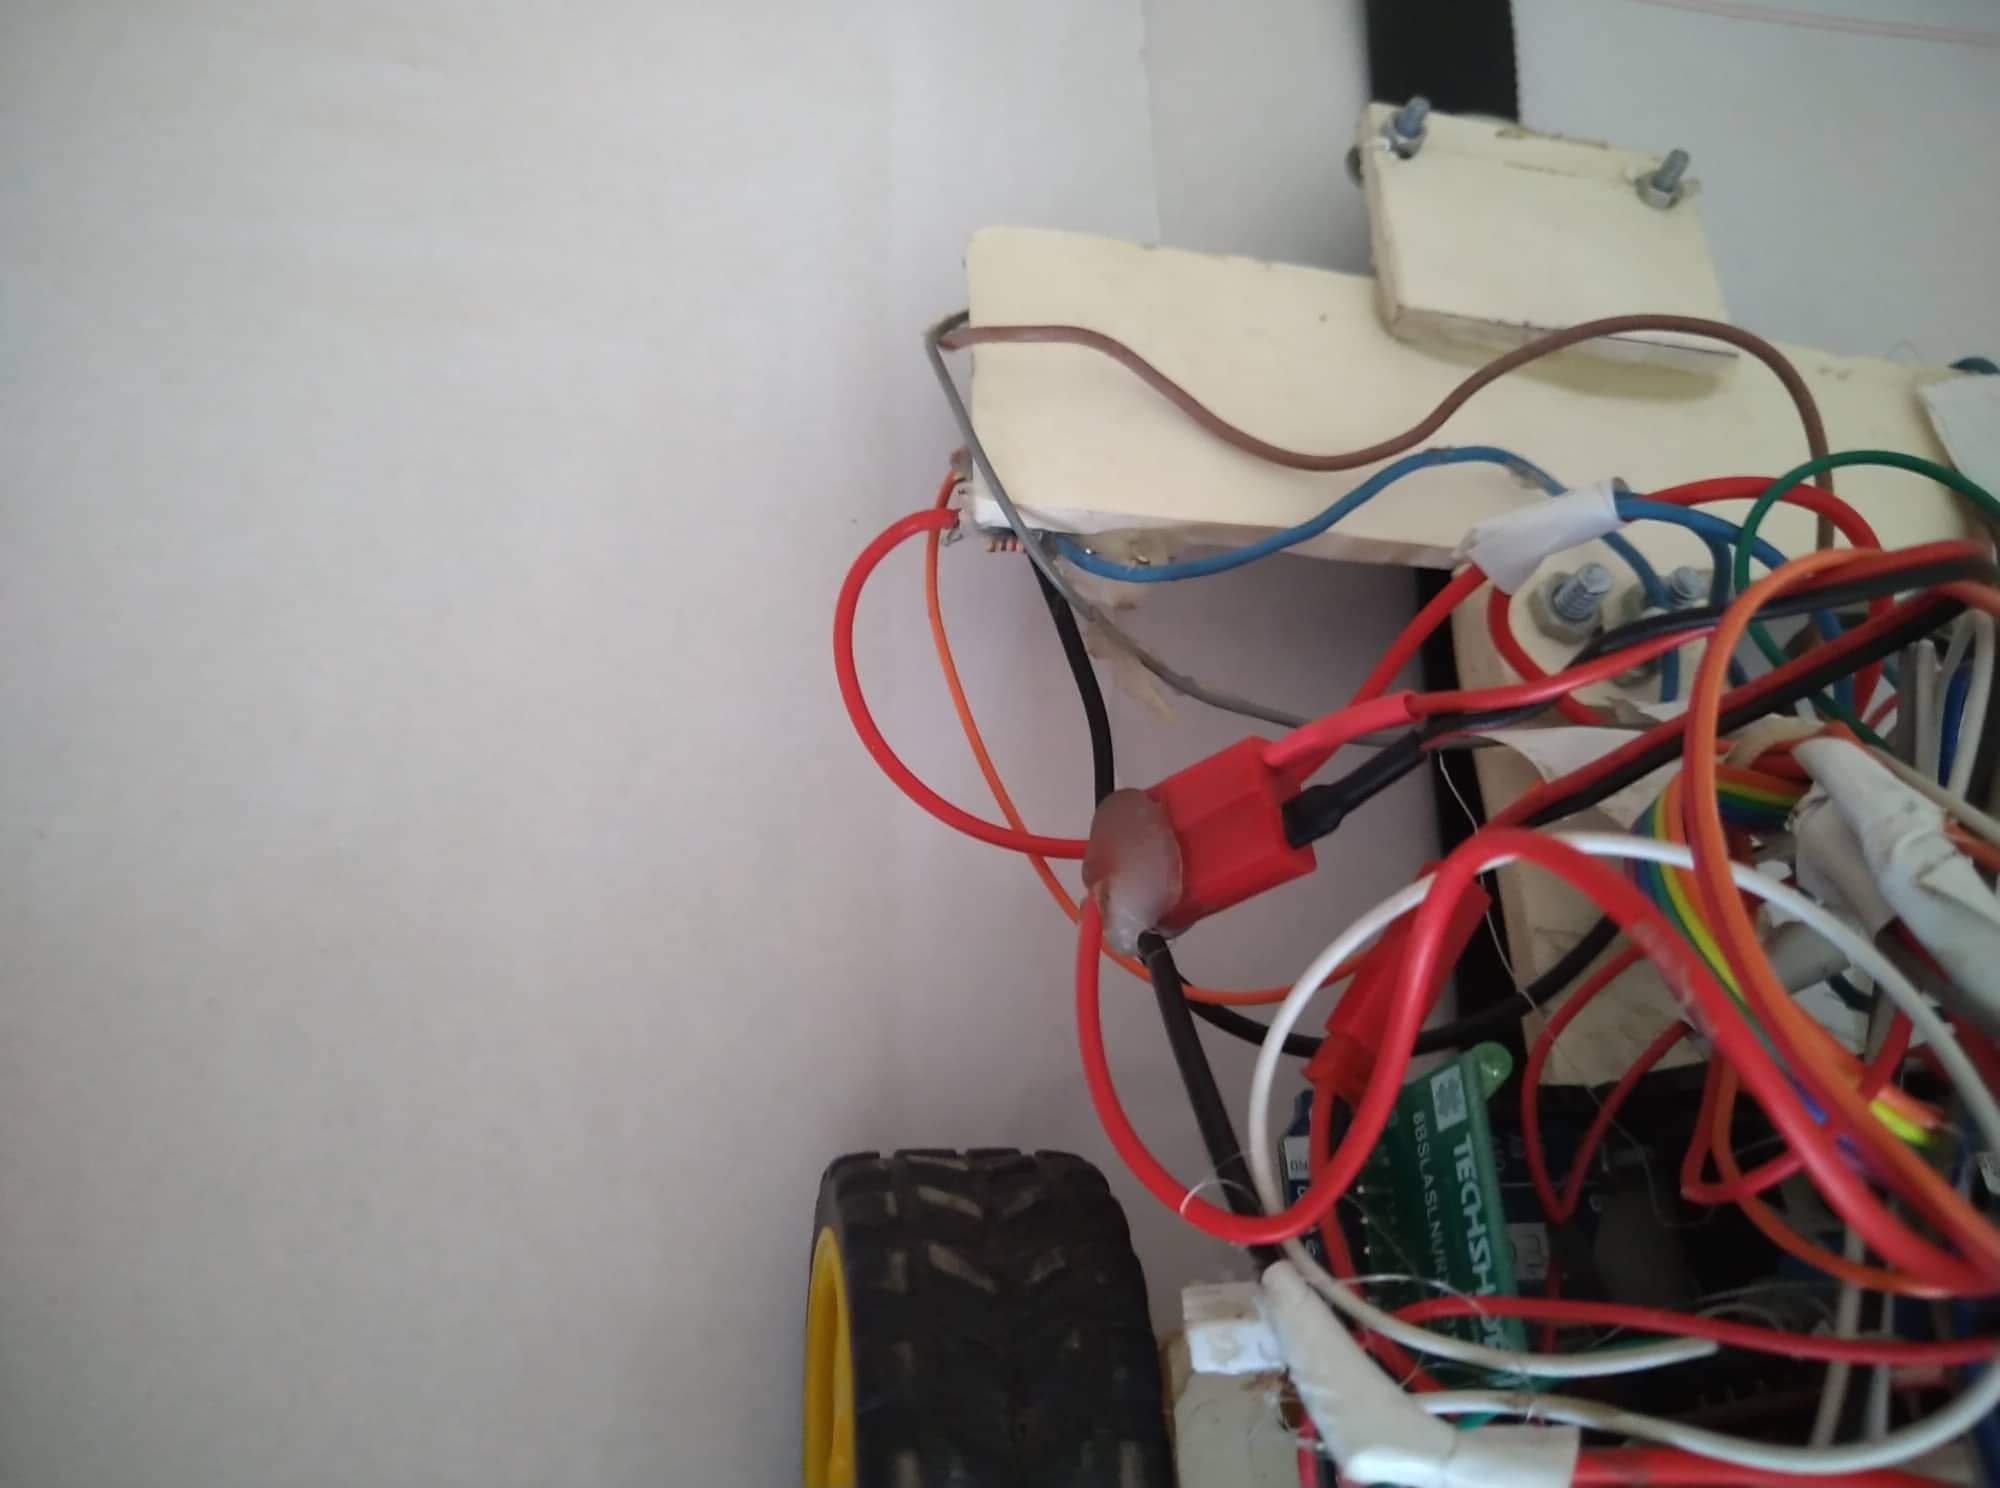
\includegraphics[scale=0.30]{line_follower}
		\caption{A Simple Line Follower for Simulation}
	\end{figure}
	\vline
       
    \chapter{Conclusion}
Our language processing task also have needed some fundamental modifications. We still worked with English language but we hope to work for Bengali language. Processing Bengali language in a computational environment is a challenging task. We've have to work with unicode. As Bengali language have more difficult syntax then English language so one of our core challenging task still remain.\\

Further its difficult to work with Bengali language as there are not enough Bengali language datasets for such computational tasks. We might have to make our own dataset for training the fundamental models that we've used in this task.\\

For processing Language and extracting necessary information in this case, determining which is desired destination in a given natural language instruction we used very basic machine learning model without any hyper-parameter tuning. So we didn't get enough good result but we hope to use more advance models or neural networks that we still didn't explore much.\\

We worked with basic reinforcement learning algorithm which is not much efficient that we aimed for this project. In the upcoming advance version of this project, we aim to deploy one or more machine learning models to generate necessary navigation commands from given natural language instruction.\\

The reinforcement learning algorithm that we've used here, in a known environment it works properly and efficiently. But with the increase of environment this algorithms becomes slower. So for a complex environment this algorithm is not much suitable. As our environment is still not much complex so our algorithm will work properly here.\\

Our simulation environment is still very simple and we used this currently for demonstration purpose only. This environment represents nothing of real life. We aim to design an environment that'll capable of represents a real life environment.\\

We've studied several papers and tested various technical issues. So apparently our task seems very simple but the implication of our endeavor will be visible very soon.	  
	

	\bibliographystyle{plain}
	\bibliography{procite}
\end{document}